% kapitel2.tex
\chapter{Ergebnisse und Evaluierung}
\label{chapter:evaluation}

Hier werden die Ergebnisse von den trainierten Modellen gezeigt und diskutiert. Alle Ergebnisse wurden mit der folgenden Hardware mit diesen Komponenten erstellt: Zwei $Intel^{\textregistered} Xeon^{\textregistered}$ CPU E5-2650 @ 2.20GHz Prozessoren mit 112 Gb Arbeitsspeicher. Außerdem besitzt die Hardware eine Grafikkarte vom Typ NVIDIA GeForce GTX 1080 mit 8Gb Speicher.



\section{Ergebnisse}

Mithilfe der Genauigkeit und der Verlustfunktion können Aussagen darüber getroffen werden, wie gut die Modelle trainiert wurden. In diesem Abschnitt wird die Frage mittels Grafiken geklärt, ob eine Überanpassung beziehungsweise Unteranpassung stattgefunden hat. Des Weiteren werden die Ergebnisse der Modelle, die auf den Tomatendatensatz angewendet wurden, gezeigt.

\subsection{Auswertung des 5-Klassen-Modells}

In der Abbildung \ref{eval_acc_loss_5} erreichen die beiden Graphen die 96. Epoche. Das Training wurde in 

\begin{figure}[h!]
	
	\hfill
	\subfigure{
		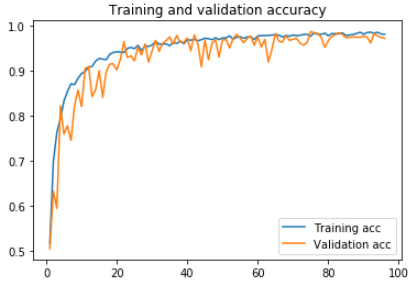
\includegraphics[width=0.44\textwidth]{model/final_model/final_model_acc.PNG}}
	\hfill
	\subfigure{
		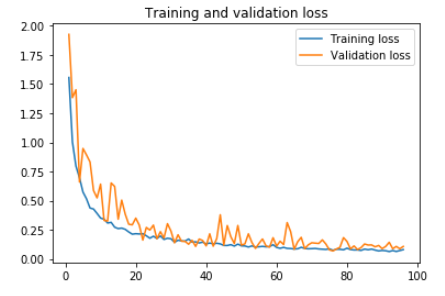
\includegraphics[width=0.48\textwidth]{model/final_model/final_model_loss.PNG}}
	\hfill
	\caption{Die linke Abbildung zeigt die Genauigkeit des Modells. Die andere Abbildung visualisiert die Werte von der Verlust-Funktion in der jeweiligen Epoche (eigene Darstellung).
	}
	\label{eval_acc_loss_5}
\end{figure}

\newpage
der 76. Epoche abgebrochen und hat eine Genauigkeit von 98.51\%. Da die beiden Graphen nah beieinander liegen, kann hier eine Über- und Unteranpassung ausgeschlossen werden. Des Weiteren stagnieren die Werte der Loss-Funktion auf dem Trainings- und Validationsdatensatz, so dass kein Anzeichen für eine Über- und Unteranpassung vorliegt.




In der Abbildung \ref{final_model_cm} ist klar zu erkennen, dass alle Krankheiten in über 98\% der Fälle korrekt klassifiziert wurden. Des Weiteren können alle Krankheiten ausgehend von einem gesunden Blatt unterschieden werden. Lediglich die Krautfäule (late blight) wurde genau einmal falsch als ein gesundes Blatt erkannt. Die Unterscheidung zwischen der Krautfäule (late blight) und Dürrfleckenkrankheit (early blight) kann in der Größenordnung von etwa fünf bis sechs Fehlklassifizierung liegen. Darüber hinaus weist das Modell zwei Fehlklassifizierungen zwischen der Samtfleckenkrankheit (leaf mold) und Dürrfleckenkrankheit (early blight) auf.

\begin{figure}[h!]
	\centering
	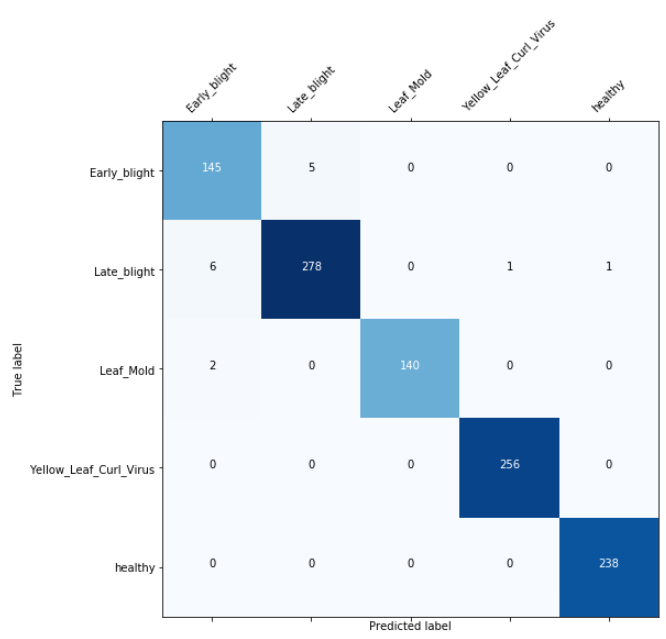
\includegraphics[width=0.83\textwidth]{model/final_model/final_model_cm.PNG}
	\caption{Veranschaulichung von Klassifizierungen des 5-Klassen Modells (eigene Darstellung).}
	\label{final_model_cm}
\end{figure}

\newpage
\subsection{Auswertung des Voters}

In diesem Unterabschnitt werden jeweils die Ergebnisse der Modelle, die für zwei Krankheiten trainiert wurden, diskutiert. Anschließend wird eine Wahrheitsmatrix gezeigt, die das Ergebnis der drei Modelle mithilfe des Voting-Verfahrens veranschaulicht. Die Performanz des Voters wird dann mit den einzelnen Modellen verglichen.


\subsubsection{Modell 1}

Die Abbildung \ref{eval_acc_loss_voter1} zeigt, dass die Genauigkeit und die Verluste unter großen Schwankungen stehen. Der Verlauf des Validationsdatensatzes weist eine alternierende Struktur auf. Das Training wurde in der 35. Epoche abgebrochen, da die Werte zu dieser Epoche auf der selben Höhe liegen und keine weiteren Verbesserungen auftraten. Dort befindet sich auch der minimalste Verlust. Die Werte der Loss-Funktion werden mit steigender Epochenanzahl nicht kleiner. Letztendlich besitzt das Modell eine Genauigkeit von 97.94\%. Des Weiteren ist hier eine Überanpassung erkennbar, weil der Verlauf des Validationsdatensatzes in der rechten Abbildung oberhalb des Trainingsverlaufs ist.


\begin{figure}[h!]
	
	\hfill
	\subfigure{
		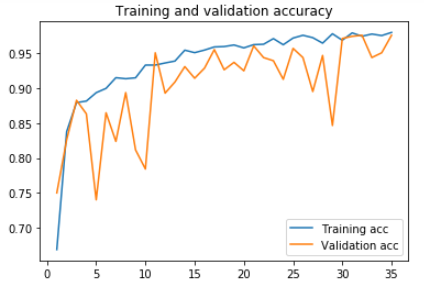
\includegraphics[width=0.48\textwidth]{model/voter1/voter1_acc.PNG}}
	\hfill
	\subfigure{
		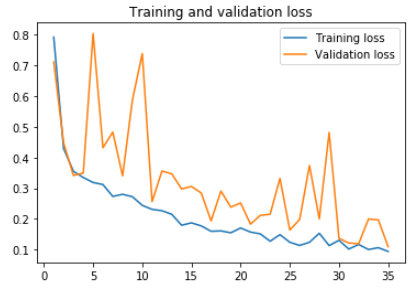
\includegraphics[width=0.47\textwidth]{model/voter1/voter1_loss.PNG}}
	\hfill
	\caption{Die Genauigkeit des ersten Modells ist in der linken Abbildung visualisiert. Die Verläufe der beiden Datensätze liegen nah beieinander. Die Werte der Verlust-Funktion von dem Validationsdatensatz nähern sich mit steigender Epochenanzahl an den Trainingsdatensatz an. Dies wird in der rechten Abbildung gezeigt (eigene Darstellung).
	}
	\label{eval_acc_loss_voter1}
\end{figure}

In Abbildung \ref{voter1_cm} wird eine Matrix veranschaulicht, die die Performance der Klassifizierung darstellt. Gesunde Blätter werden in diesem Modell stets richtig klassifiziert. Ausgehend von der Krautfäule existieren zwei Fehlklassifizierung. Diese werden als Dürrfleckenkrankheit (early blight) wahrgenommen. Blätter von der Dürrfleckenkrankheit werden vier Mal als Krautfäule erkannt.

\begin{figure}[h!]
	\centering
	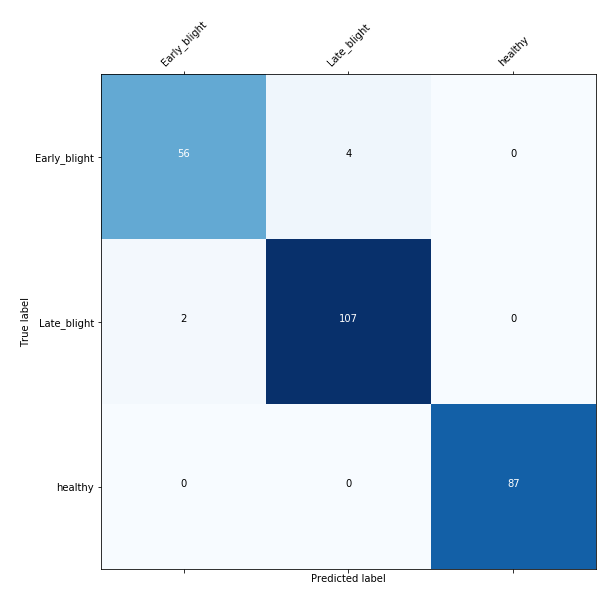
\includegraphics[width=0.8\textwidth]{model/voter1/voter1_cm.PNG}
	\caption{Veranschaulichung von Klassifizierungen des ersten Voter-Modells (eigene Darstellung).}
	\label{voter1_cm}
\end{figure}

\newpage
\subsubsection{Modell 2}

Auch das zweite Modell hat eine leichte Überanpassung. In der Abbildung \ref{eval_acc_loss_voter2} sind die Graphen bezüglich der Genauigkeit und der Verlustwerte abgebildet. In beiden Graphen

\begin{figure}[h!]
	
	\hfill
	\subfigure{
		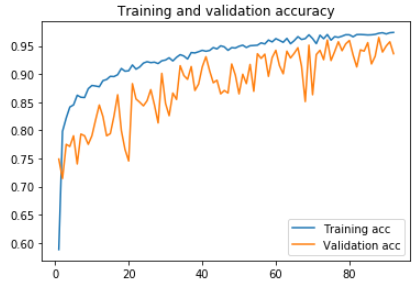
\includegraphics[width=0.48\textwidth]{model/voter2/voter2_acc.PNG}}
	\hfill
	\subfigure{
		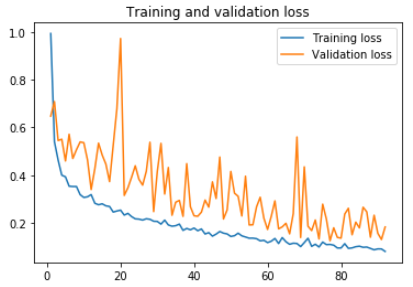
\includegraphics[width=0.48\textwidth]{model/voter2/voter2_loss.PNG}}
	\hfill
	\caption{Die linke Abbildung veranschaulicht die Genauigkeit des Modells in den jeweiligen Datensatz. Die Verlust-Werte (rechte Abbildung) liegen nicht eng beieinander (eigene Darstellung).
	}
	\label{eval_acc_loss_voter2}
\end{figure}

ist diese Überanpassung erkennbar. In der linken Abbildung ist der Verlauf des Trainingsdatensatzes oberhalb des Validationsdatensatzes. In dem rechten Graphen befindet sich der Verlauf des Validationsdatensatzes oberhalb des Trainingsdatensatzes. Außerdem weist auch hier der Validationsdatensatz einen alternierenden Verlauf an. Die beiden Graphen gehen bis zur 92. Epoche, da das Training früher abgebrochen wurde. Der minimalste Verlust wurde in der 77. Epoche gefunden und hat in dieser Epoche eine Genauigkeit von 96.54\%. Dieses Modell zu dieser Epoche legt die besten Ergebnisse vor.



Die Abbildung \ref{voter2_cm} veranschaulicht, dass alle gesunden Blätter korrekt erkannt sowie nicht als Krankheit verwechselt werden. Solche Ergebnisse zeigt auch die Dürrfleckenkrankheit (early blight). Lediglich erkennt das Modell zweimal die Krankheit Krautfäule (late blight) als Dürrfleckenkrankheit (early blight).


\begin{figure}[h!]
	\centering
	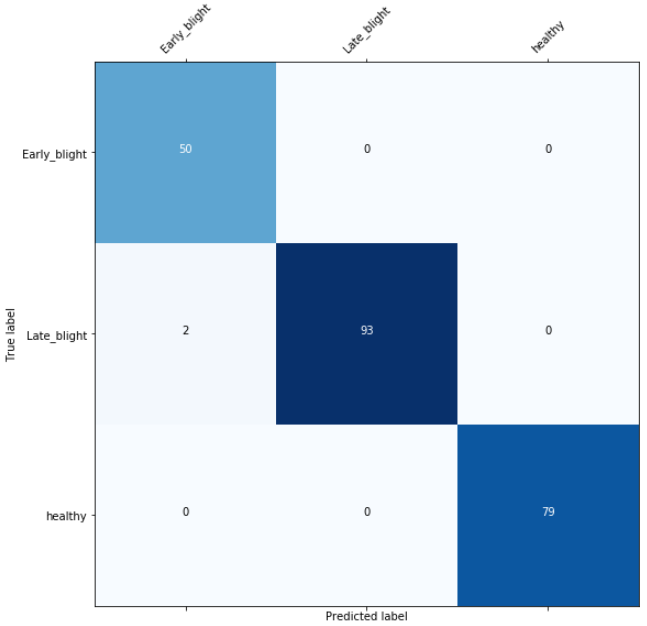
\includegraphics[width=0.83\textwidth]{model/voter2/voter2_cm.PNG}
	\caption{Veranschaulichung von Klassifizierungen des zweiten Voter-Modells (eigene Darstellung).}
	\label{voter2_cm}
\end{figure}


\subsubsection{Modell 3}

In der Abbildung \ref{eval_acc_loss_voter3} werden die beiden Graphen bezüglich der Genauigkeit und der Verluste bis zur 79. Epoche visualisiert. Die Genauigkeit und die Loss-Werte des Validationsdatensatzes verlaufen in den ersten 40 Epochen alternierend mit großem Abstand zu dem Trainingsdatensatz. Ab der 40. Epoche nähern sich die beiden Datensätze an.

\begin{figure}[h!]
	
	\hfill
	\subfigure{
		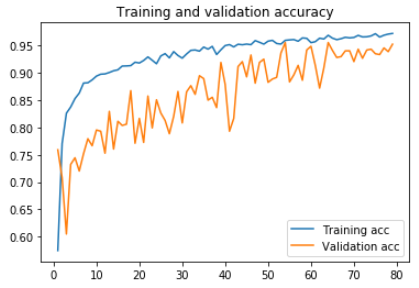
\includegraphics[width=0.48\textwidth]{model/voter3/voter3_acc.PNG}}
	\hfill
	\subfigure{
		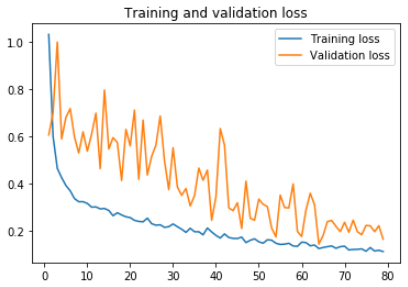
\includegraphics[width=0.48\textwidth]{model/voter3/voter3_loss.PNG}}
	\hfill
	\caption{Die linke Abbildung zeigt, dass sich die Genauigkeit des Modells auf dem Validationsdatensatz mit steigender Epochenanzahl an den Trainingsdatensatz annähert. Die Verlust-Funktion zeigt das selbe Verhalten in der rechten Abbildung (eigene Darstellung).
	}
	\label{eval_acc_loss_voter3}
\end{figure}

Dieser Effekt ist bei den beiden Grafiken zu sehen. In der 64. Epoche, in der das

\begin{figure}[h!]
	\centering
	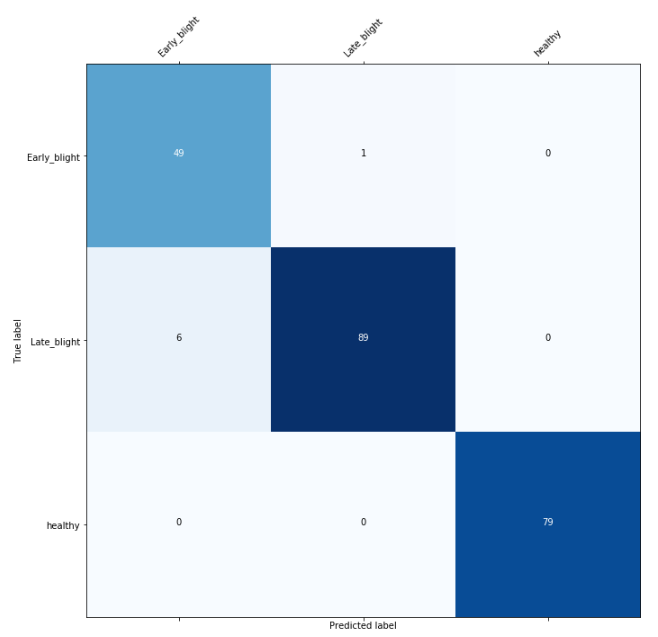
\includegraphics[width=0.75\textwidth]{model/voter3/voter3_cm.PNG}
	\caption{Veranschaulichung von Klassifizierungen des dritten Voter-Modells (eigene Darstellung).}
	\label{voter3_cm}
\end{figure}
~\newline
Training abgebrochen wurde, hat das dritte Modell die höchste Genauigkeit mit 96.62\%. Die Struktur der Graphen zeigen eine Stagnierung mit steigender Epochenanzahl.



Des Weiteren hat das Modell eine leichte Überanpassung. Die Genauigkeit liegt bei dem Trainingsdatensatz höher als der Validationsdatensatz. Weiterhin sind die Verlustwerte bei dem Trainingsdatensatz geringer als der Validationsdatensatz.

Die Abbildung \ref{voter3_cm} visualisiert die Ergebnisse der Klassifikation mit dem Testdatensatz. Es existiert keine Verwechslung mit gesunden Blättern. Des Weiteren werden diese auch alle korrekt als gesunde Blätter klassifiziert. Die Dürrfleckenkrankheit (early blight) wird genau einmal falsch als Krautfäule (late blight) erkannt. Mit sechs Fehlklassifizierungen zeigt die Klasse \glqq late blight\grqq, dass Fehlklassifizierungen mit der Dürrfleckenkrankheit (early blight) auftreten können.


\subsubsection{Wahrheitsmatrix mit den drei Modellen}

In der Abbildung \ref{voter_combined} zeigt sich, dass der Voter die Ergebnisse der einzelnen Modelle verbessern kann. Nur das zweite Modell weist ohne die Hilfe des Voters bessere Ergebnisse auf.

\begin{figure}[h!]
	\centering
	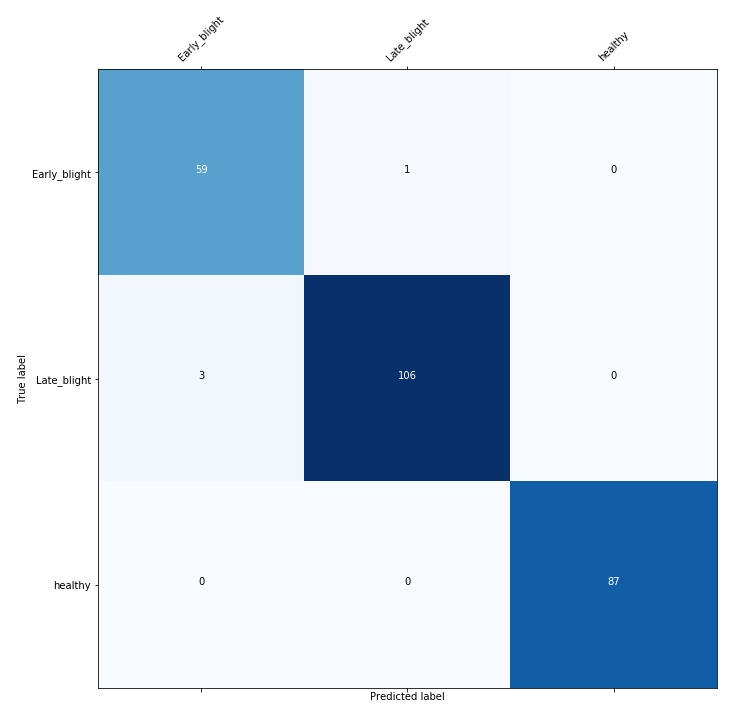
\includegraphics[width=0.73\textwidth]{bilder/voter.PNG}
	\caption{Veranschaulichung von Klassifizierungen mit drei Modellen, die mithilfe von einem Voting-Verfahren bestimmt wurden (eigene Darstellung).}
	\label{voter_combined}
\end{figure}


Das zweite Modell hat lediglich zwei Fehlklassifikation. Der Voter klassifiziert gegenüber dem ersten Modell deutlich besser die Dürrfleckenkrankheit (early blight). Allerdings ist die Erkennung der Krautfäule (late blight) mit dem ersten Modell minimal besser. Hier verringert sich die Anzahl der Fehlklassifizierung von drei auf zwei. Das dritte Modell hat bei der Erkennung der Krautfäule (late blight) sechs Fehlklassifizierungen. Der Voter erkennt hierbei nur drei Exemplare falsch.


\subsection{Auswertung des transfergelernten Modells}


Die Abbildung \ref{eval_acc_loss_transfer} zeigt den Verlauf des Trainings in dem Aspekt der Genauigkeit und der Verlust-Funktion. Dieser geht bis zu der 103. Epoche. Der geringste Verlustwert wurde in der 68. Epoche gefunden und das Modell besitzt eine Genauigkeit von 71.1\%. Die Graphen in den beiden Abbildungen liegen nicht eng beieinander. Des Weiteren ist dieses Modell das einzige Modell mit einer Unteranpassung. Die Unteranpassung lässt sich daran erkennen, dass die Genauigkeit des Trainingsdatensatzes unterhalb des Validationsdatensatzes liegt. Außerdem sind die Verlustwerte bei dem Validationsdatensatz geringer als bei dem Trainingsdatensatz.

\begin{figure}[h!]
	\hfill
	\subfigure{
		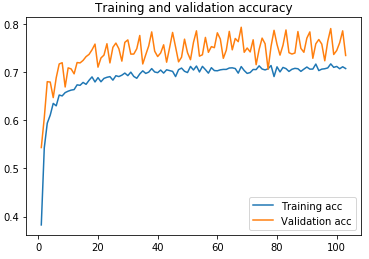
\includegraphics[width=0.48\textwidth]{model/transfer/acc.png}}
	\hfill
	\subfigure{
		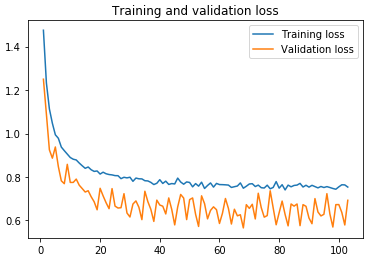
\includegraphics[width=0.48\textwidth]{model/transfer/loss.png}}
	\hfill
	\caption{Genauigkeit (links) und Loss-Funktion (rechts) des transfergelernten Modells. In beiden Graphiken ist die Unteranpassung sichtbar (eigene Darstellung).
	}
	\label{eval_acc_loss_transfer}
\end{figure}



In der Abbildung \ref{transfer_confusion_matrix} sind die Schwächen des Modells klar zu erkennen. Größtenteils wird die Krankheit korrekt erkannt. Dennoch treten Fehlklassifizierungen auf. Bei der Klasse \glqq early blight\grqq~gibt es keine Verwechslung mit gesunden Blättern. Allerdings werden zwei Mal gesunde Blätter als die Dürrfleckenkrankheit (early blight) erkannt. Des Weiteren hat diese Klasse leichte Schwierigkeiten mit der Klasse \glqq late blight\grqq. Die Anzahl der Fehlklassifikation liegt bei neun. Die restlichen zwei Klassen haben maximal fünf Fehlklassifikationen.

Die Klasse \glqq late blight\grqq~ hat Schwierigkeiten mit den Klassen \glqq early blight\grqq~und \glqq leaf mold\grqq. Mit 18 beziehungsweise 10 Fehlerkennung ist die Fehlerrate recht hoch. Am wenigsten hat die Klasse Probleme mit der Krankheit \glqq TYLCV\grqq.

Die beste Performance bezüglich der Klassifikation hat die Klasse \glqq leaf mold\grqq. Diese hat höchstens zwei Fehlklassifkationen in allen Klassen. Die schlechtesten Ergebnisse sind von der Klasse \glqq TYLCV\grqq. Diese zeichnet sich durch eine hohe Fehlerkennung mit der Dürrfleckenkrankheit (early blight), nämlich 26, aus.
Auch bei dem Vergleich mit den anderen Klassen schneidet die Klasse \glqq TYLCV\grqq deutlich schlechter ab. Nur die Erkennung von gesunden Blättern schlägt genau drei Mal fehl. Die Klasse der gesunden Blätter hat mit fünf Fehlerkennungen bei der Klasse \glqq leaf mold\grqq~ leichte Defizite.

\begin{figure}[h!]
	\centering
	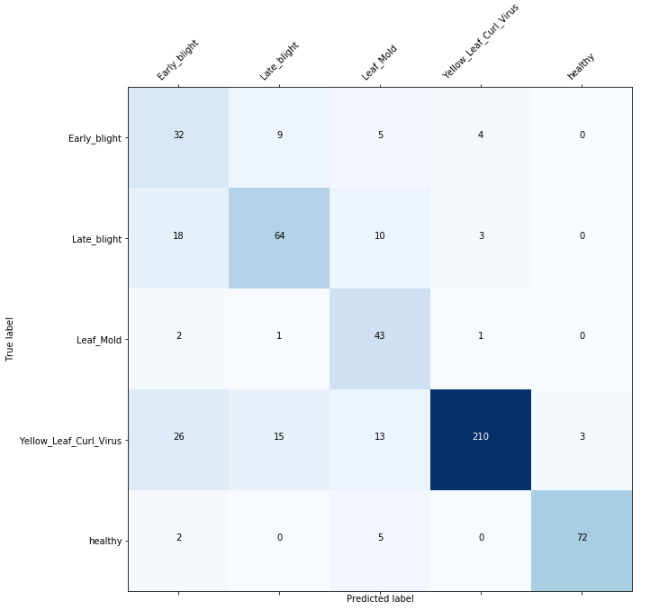
\includegraphics[width=0.83\textwidth]{model/transfer/confusion_matrix.PNG}
	\caption{Veranschaulichung von Klassifizierungen des Modells, welches durch Transfer Learning gelernt hat (eigene Darstellung).}
	\label{transfer_confusion_matrix}
\end{figure}


\section{Evaluierung}

Manche Blattkrankheiten, zum Beispiel die Dürrfleckenkrankheit und die Krautfäule, treten nicht nur bei Tomaten auf. Andere Nachtschattengewächse beispielsweise Kartoffeln sind auch von diesen Krankheiten betroffen. In diesem Abschnitt werden diese Krankheiten auf den Blättern von Kartoffeln mit den Modellen, die eigentlich für Tomaten vorgesehen sind, vorhergesagt. In Abbildung \ref{potatoes_combined} ist eindeutig zu sehen, dass die trainierten Modelle auf dem Kartoffeldatensatz keine gute Ergebnisse zeigen. Die Dürrfleckenkrankheit (early blight) wird am häufigsten bei allen Modellen als gesunde Blätter erkannt. Die Krautfäule (late blight) wird auch sehr häufig als gesunde Blätter klassifiziert. Des Weiteren ist die 


\begin{figure}[h!]
	\centering
	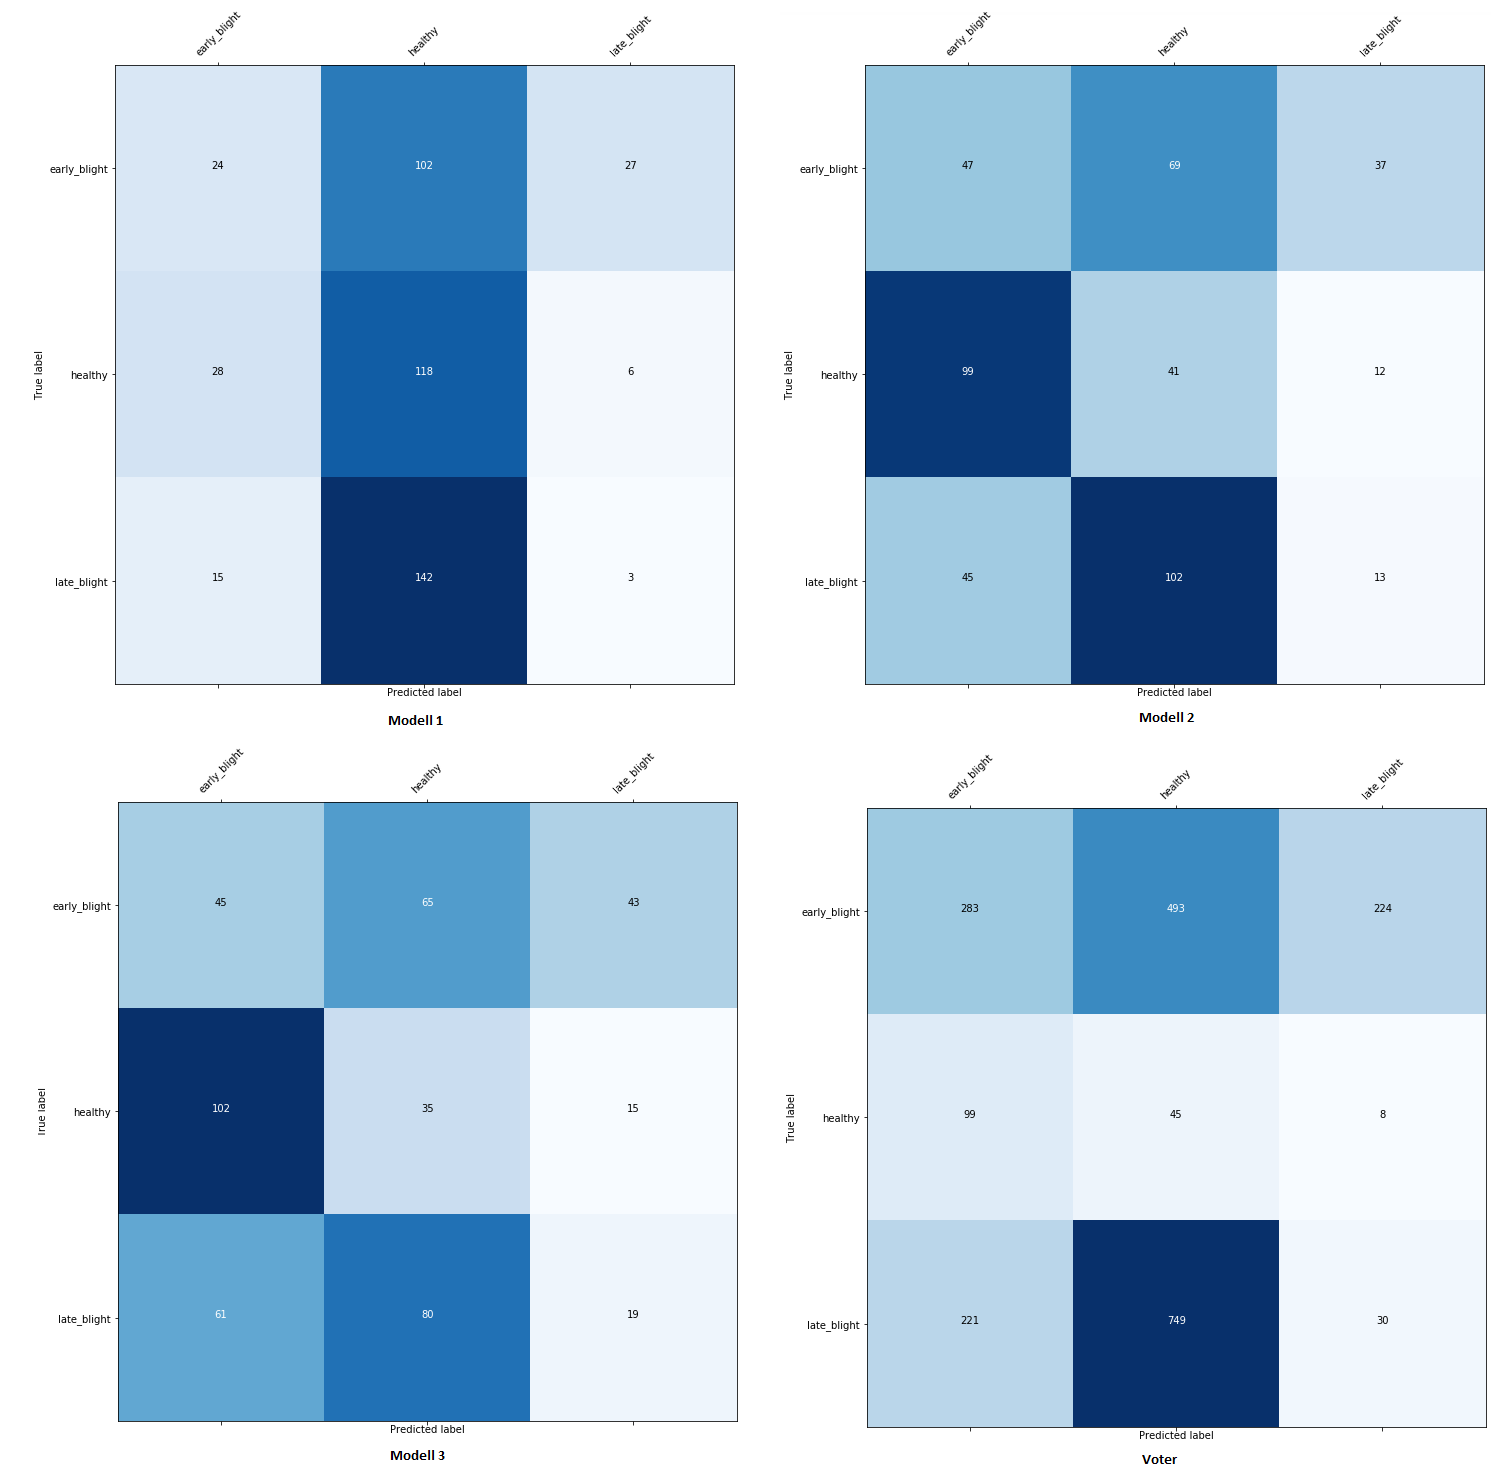
\includegraphics[width=\textwidth]{potatoes_plots/combined.PNG}
	\caption{Veranschaulichung von Klassifizierungen des Modells auf dem Kartoffeldatensatz (eigene Darstellung).}
	\label{potatoes_combined}
\end{figure}

Erkennung von Krautfäule bei allen Modellen kaum vorhanden. In dem ersten Modell wurde die Krautfäule lediglich drei Mal erkannt. In dem dritten Modell wurde diese Krankheit höchstens 19 Mal klassifiziert. Nur in dem ersten Modell werden gesunde Blätter überproportional als gesunde Blätter erkannt. Andere Modelle haben mit der Erkennung der gesunden Blätter Schwierigkeiten und erkennen gesunde Blätter oft als Dürrfleckenkrankheit (early blight). Der Voter sorgt für keine Besserung und zeigt das Verhalten wie die anderen Modelle. Eine mögliche Erklärung für diese Ergebnisse können die unterschiedliche Struktur der Blattoberfläche sowie die Form sein. Die Modelle haben nicht nur die Erkennung der Flecken gelernt, sondern auch die Struktur von dem vorliegenden Blatt.

In den Abbildungen \ref{eval_pot_early} und \ref{eval_pot_late} ist klar zu sehen, dass die Aderung des Blattes beispielsweise unterschiedlich ist. Weiterhin ähneln die Blätter von Tomaten einer Pfeilspitze. Bei Kartoffeln ist die Form eher oval.


\begin{figure}[t!]
	\hfill
	\subfigure{
		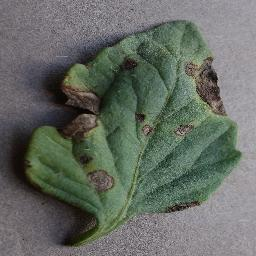
\includegraphics[width=0.43\textwidth]{potatoes_plots/tom_early.JPG}}
	\hfill
	\subfigure{
		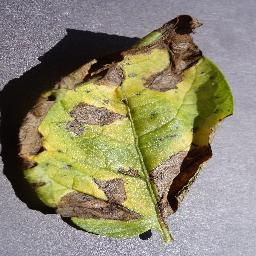
\includegraphics[width=0.43\textwidth]{potatoes_plots/pot_early.JPG}}
	\hfill
	\caption{Visualisierung der Dürrfleckenkrankheit bei Tomaten (links) und Kartoffeln (rechts) (eigene Darstellung).
	}
	\label{eval_pot_early}
\end{figure}

\begin{figure}[h!]
	\hfill
	\subfigure{
		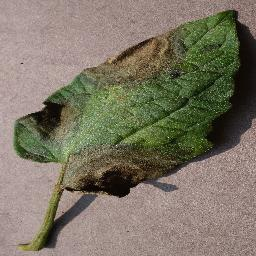
\includegraphics[width=0.43\textwidth]{potatoes_plots/tom_late.JPG}}
	\hfill
	\subfigure{
		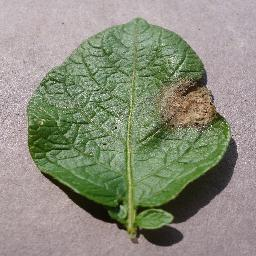
\includegraphics[width=0.43\textwidth]{potatoes_plots/pot_late.JPG}}
	\hfill
	\caption{Visualisierung der Krautfäule bei Tomaten (links) und Kartoffeln (rechts) (eigene Darstellung).
	}
	\label{eval_pot_late}
\end{figure}















\newpage
\section{Visualisierung}

Die Klassenentscheidung von neuronalen Netzen ist auf den ersten Blick nicht ganz klar, weil grundsätzliche Visualisierungen den Benutzern nicht angezeigt werden. Dadurch entsteht der Eindruck, dass neuronale Netze wie eine Blackbox wirken. Durch Visualisierungen können die Entscheidungen von neuronalen Netzen nachvollziehbar dargestellt werden. In diesem Abschnitt werden die Aktivierungswerte in den Faltungschichten visualisiert. Des Weiteren können die Aktivierungswerte in einer Heatmap dargestellt werden. Alle Abbildungen von jeder Krankheit und gesunden Blättern werden im Anhang A-E auf den Seiten \pageref{anahnga} - \pageref{anahngd} bereitgestellt.


\begin{figure}[h!]
	\hfill
	\subfigure{
		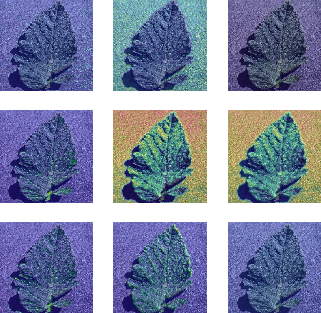
\includegraphics[width=0.44\textwidth]{visualisierungen/healthy/heatmap_ohne/cropped_ohne.png}}
	\hfill
	\subfigure{
		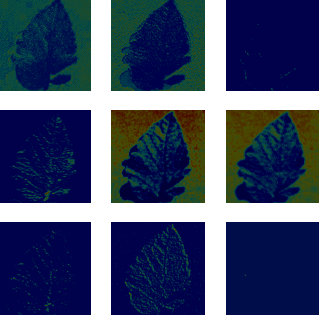
\includegraphics[width=0.43\textwidth]{visualisierungen/healthy/heatmap_mit/cropped_mit.png}}
	\hfill
	\caption{Die linke Darstellung hat keine Normierung der Farbwerte. Das rechte Bild mit der Normierung zeigt schwache Aktivierungswerte deutlicher an (eigene Darstellung).
	}
	\label{vis_normalised_rgb}
\end{figure}


Angemerkt sei, dass die Darstellung mit normierten Farbwerte visualisiert wird. Die Abbildung \ref{vis_normalised_rgb} zeigt deutlich, dass die Aktivierungswerte in der normierten Grafik (rechts) erkennbarer als die nicht normierten Bilder sind. Das linke Bild zeigt zwar das Hintergrundbild, allerdings sind schwache Aktivierungswerte kaum erkennbar.

\subsection{Gesunde Blätter}

Die Abbildung \ref{healthy_sample} wird als Ausgangsbild für die Visualisierung benutzt. Die dritte Faltungschicht ist für dieses Beispiel ideal, da die Visualisierung noch Strukturen des Blattes aufweist (s. Abbildung \ref{healthy6}). 
\begin{figure}[h!]
	\centering
	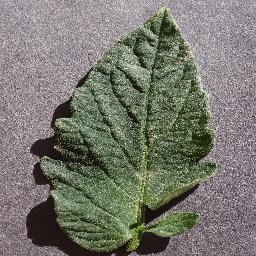
\includegraphics[width=0.5\textwidth]{visualisierungen/healthy/healthy_sample.jpg}
	\caption{Das Beispielbild für die Visualisierung von gesunden Blättern (eigene Darstellung).}
	\label{healthy_sample}
\end{figure}

\newpage
Die Aderung und die Umrandung des Blattes ist noch in der Abbildung erkennbar. Außerdem hat das 5-Klassen Modell nur vereinzelt den Hintergrund gelernt. Insgesamt haben 51 Filter auf das Eingangsbild nicht reagiert. Die vierte und fünfte Faltungschicht, die sich in dem Anhang befinden, zeigen abstrakte kleine Konstrukte, die nicht genau zuordenbar sind.

\begin{figure}[h!]
	\centering
	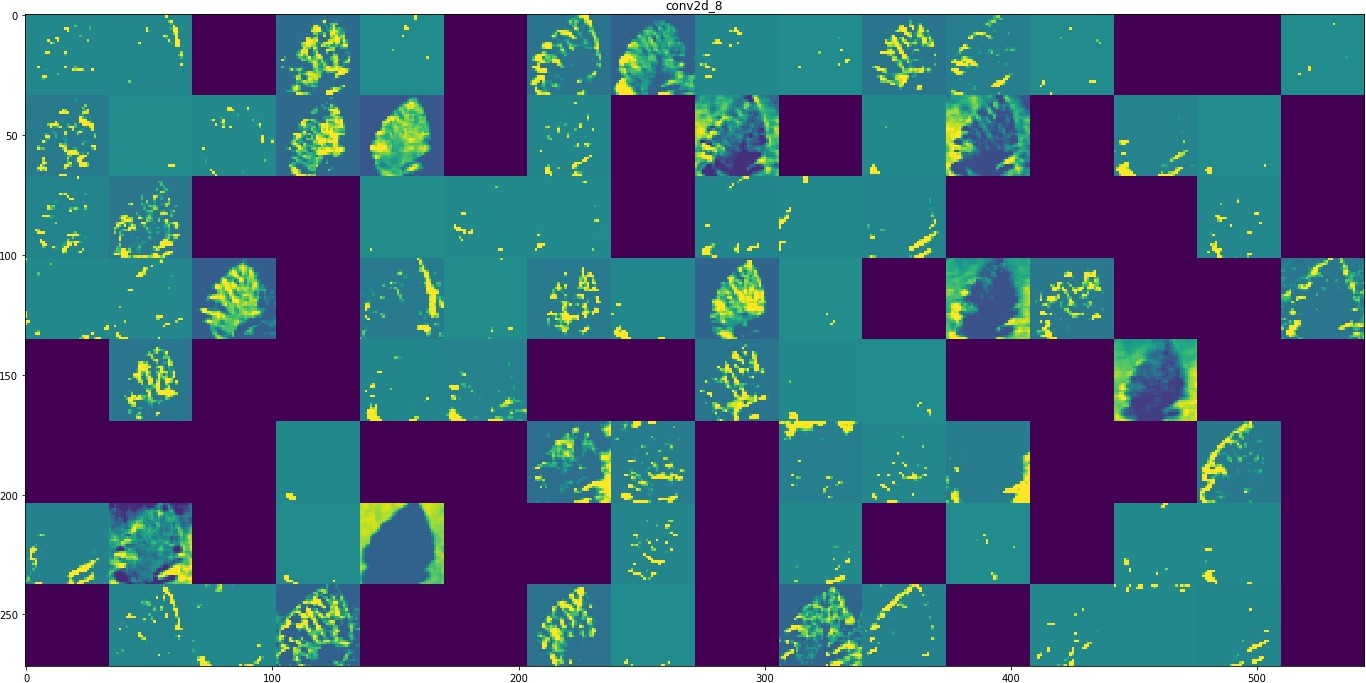
\includegraphics[width=\textwidth]{visualisierungen/healthy/activation/healthy6.JPG}
	\caption{Visualisierung der Aktivierungswerte in der dritten Faltungschicht von gesunden Blättern (eigene Darstellung).}
	\label{healthy6}
\end{figure}

In der Heatmap \ref{conv2d_8_healthy} ist klar zu sehen, dass zwei Filter den Hintergrund gelernt haben. Außerdem sind die Konzentrationen großteils an dem Rand des Blattes angesiedelt und treten vereinzelt auf. In der letzten Faltungschicht sind die Konzentrationen signifikant größer und mittig positioniert (s. Abbildung \ref{conv2d_10_heat}).

\begin{figure}[h!]
	\centering
	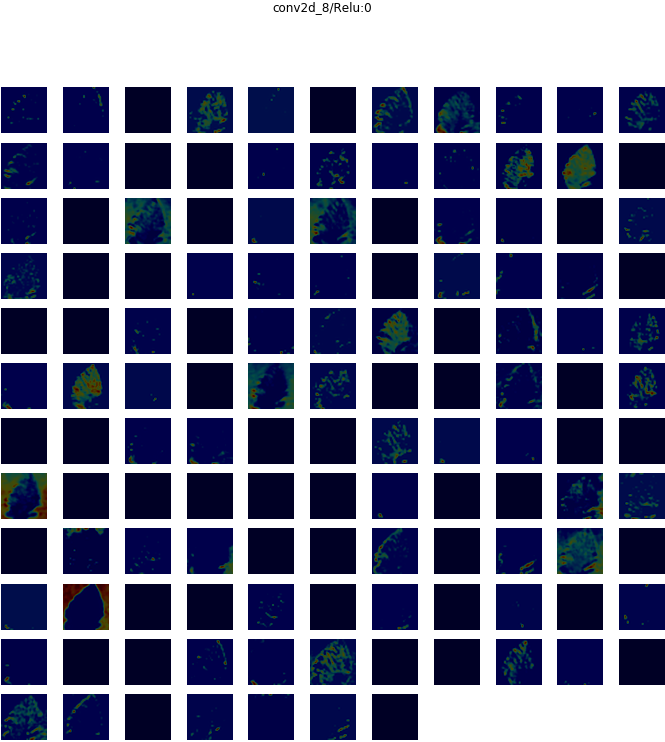
\includegraphics[width=\textwidth]{visualisierungen/healthy/heatmap_mit/conv2d_8.png}
	\caption{Visualisierung der Aktivierungswerte als Heatmap in der dritten Faltungschicht von gesunden Blättern (eigene Darstellung).}
	\label{conv2d_8_healthy}
\end{figure}

\newpage
\subsection{Dürrfleckenkrankheit}

Die erste Krankheit, die hier visualisiert wird, ist die Dürrfleckenkrankheit. Die Abbildung \ref{early_visual} zeigt das Ausgangsbild. Das Blatt hat vermehrt Flecken auf der rechten Seite. Diese verlaufen an der Hauptaderung des Blattes entlang. In der unteren linken Ecke befinden sich vereinzelte Flecken, die sowohl an der Hauptaderung als auch an dem Rand des Blattes liegen. Des Weiteren weist das Bild gelbe Bereiche in dem unteren rechten Bereich auf.


%\begin{figure}[h!]
%	\centering
%	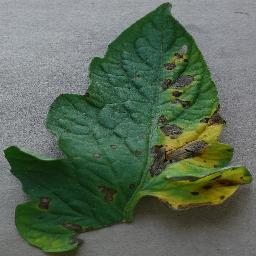
\includegraphics[width=0.45\textwidth]{visualisierungen/early/early.jpg}
%	\caption{Das Beispielbild für die Visualisierung der Dürrfleckenkrankheit (eigene Darstellung).}
%	\label{early_visual}
%\end{figure}

\begin{wrapfigure}{r}{8cm}
	\centering
	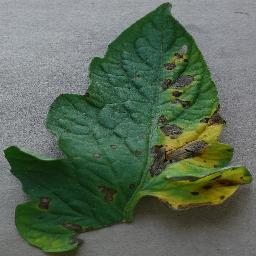
\includegraphics[width=0.45\textwidth]{visualisierungen/early/early.jpg}%
	\caption{Das Beispielbild für die Visualisierung der Dürrfleckenkrankheit (eigene Darstellung).}
	\label{early_visual}
\end{wrapfigure}

In der dritten Faltungschicht (s. Abbildung \ref{early_visual_act}) hat das Modell einige Male den Hintergrund gelernt. Großteil der Aktivierungen finden in der rechten Hälfte an der Hauptaderung statt. Das Modell ist auch in der Lage, gelbe Flächen auf der rechten Seiten zu lernen. Weiterhin sind die Flecken auf der unteren linken Seite vereinzelt in der Abbildung erkennbar. 45 Filter haben in dieser Faltungschicht nicht auf das Bild angesprochen. Die vierte Faltungschicht in der Abbildung \ref{early8_anhang} zeigt dasselbe Verhalten wie in der dritten Schicht. Allerdings ist in der vierten Schicht die Reaktion deutlich erkennbarer.

\begin{figure}[h!]
	\centering
	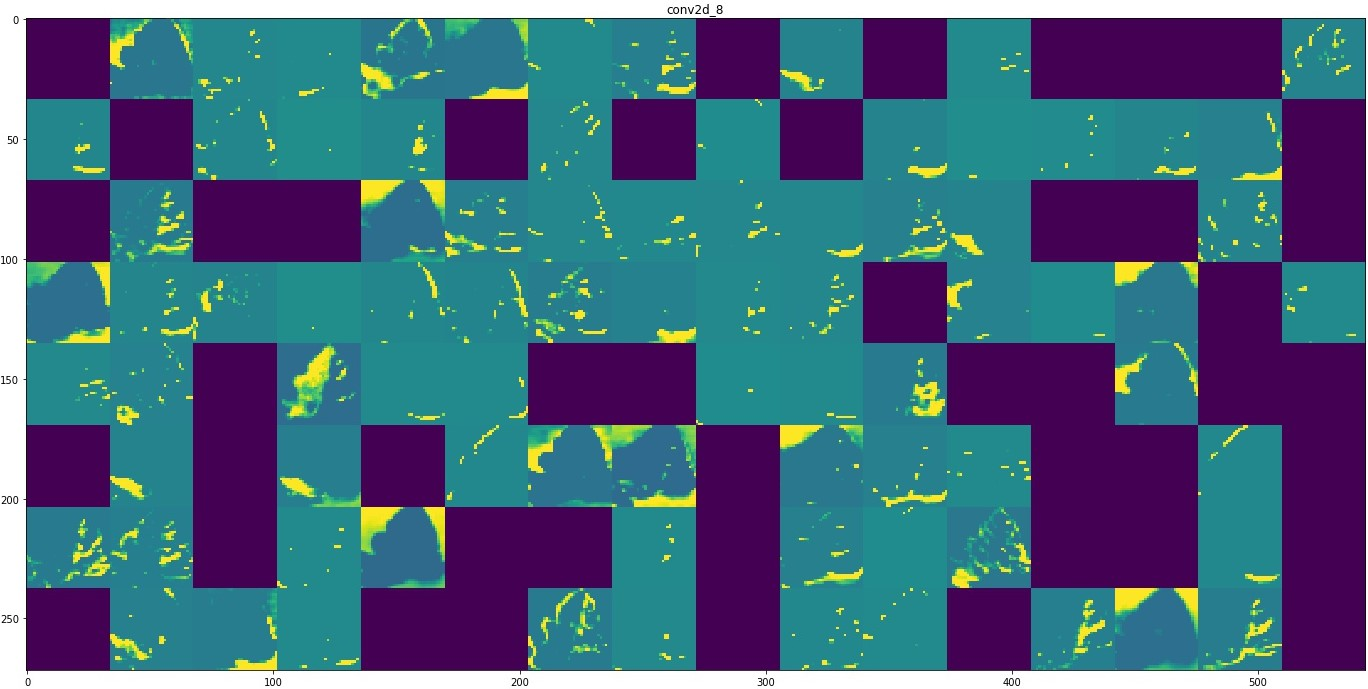
\includegraphics[width=\textwidth]{visualisierungen/early/activation/early6.JPG}
	\caption{Visualisierung der Aktivierungswerte in der dritten Faltungschicht von der Dürrfleckenkrankheit (eigene Darstellung).}
	\label{early_visual_act}
\end{figure}

Die Aktivierungswerte konzentrieren sich an Stellen, an denen die Flecken vorhanden sind (s. Abbildung \ref{conv2d_8_heat_early}). Dabei wird nicht nur die rechte Seite erkannt, sondern auch die Flecken an der unten linken Ecke. Des Weiteren lernt die nachfolgende Schicht (s. Abbildung \ref{conv2d_9_anhang}) den Hintergrund nicht mehr.

\begin{figure}[h!]
	\centering
	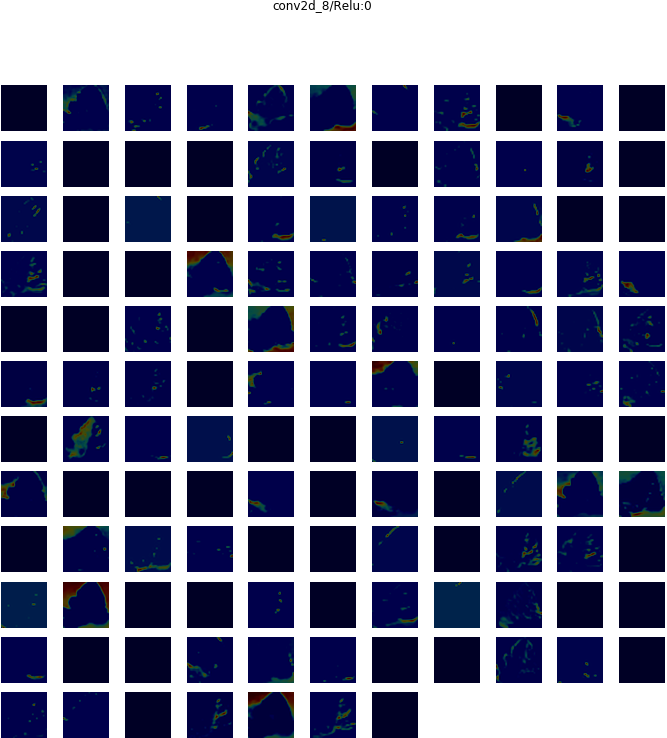
\includegraphics[width=\textwidth]{visualisierungen/early/heatmap_mit/conv2d_8.png}
	\caption{Visualisierung der Aktivierungswerte als Heatmap in der dritten Faltungschicht von der Dürrfleckenkrankheit (eigene Darstellung).}
	\label{conv2d_8_heat_early}
\end{figure}





\newpage
\subsection{Tomato Yellow Leaf Curl Virus}

Das TYLCV-Virus zeichnet sich durch die Krümmung der Blattränder sowie die Gelbfärbung des Blattes aus. Die Abbildung \ref{yellow_sample} veranschaulicht deutlich die Symptome der Viruserkrankung. Die beiden Seitenränder sind gekrümmt und in gelb verfärbt. Außerhalb der Blattränder sind manche Regionen des Blattes von der Färbung betroffen.

%\begin{figure}[h!]
%	\centering
%	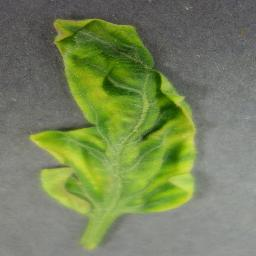
\includegraphics[width=0.5\textwidth]{visualisierungen/yellow/yellow_sample.jpg}
%	\caption{Das Beispielbild für die Visualisierung des TYLCV-Virus (eigene Darstellung).}
%	\label{yellow_sample}
%\end{figure}

\begin{wrapfigure}{r}{8cm}
	\centering
	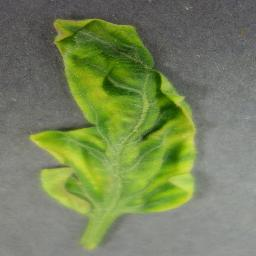
\includegraphics[width=0.45\textwidth]{visualisierungen/yellow/yellow_sample.jpg}%
	\caption{Das Beispielbild für die Visualisierung des TYLCV-Virus (eigene Darstellung).}
	\label{yellow_sample}
\end{wrapfigure}


Das Bild \ref{yellow6_act_vis} zeigt deutlich, dass die Ränder des Blattes für das Modell ein Merkmal für die Krankheit darstellt. Das Modell hat jeweils eine Seite des Randes gelernt. Einige Filter in der dritten Faltungschicht sind in der Lage, beide Seiten als Merkmale zu erkennen. Die gelben Verfärbungen, die sich außerhalb des Blattrandes befinden, werden von wenigen Filter erkannt. Des Weiteren fasst das Modell den Hintergrund des Bildes noch als Merkmal auf. Die nachfolgende Schicht hat dieses Problem nicht (s. Abbildung \ref{yellow8_anhang}). Weiterhin hat das Modell in der dritten Faltungschicht 62 inaktive Filter.

\begin{figure}[h!]
	\centering
	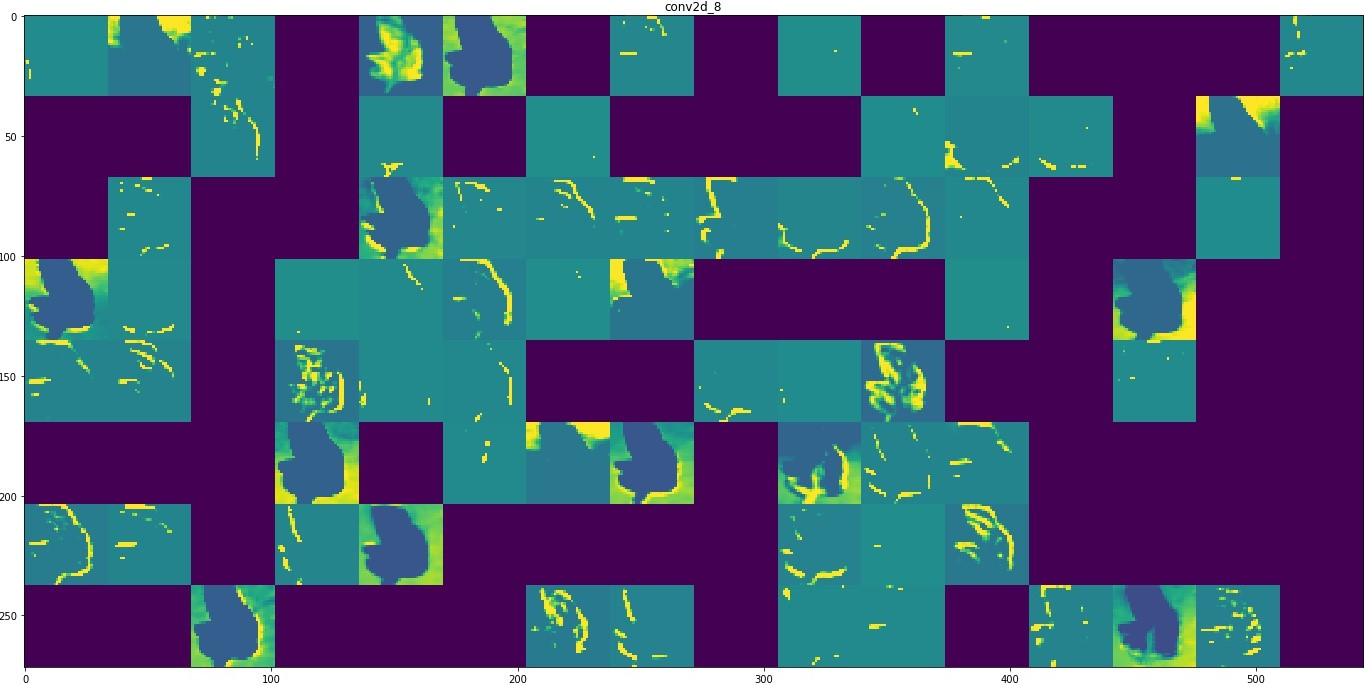
\includegraphics[width=\textwidth]{visualisierungen/yellow/activation/yellow6.JPG}
	\caption{Visualisierung der Aktivierungswerte in der dritten Faltungschicht von dem TYLCV-Virus (eigene Darstellung).}
	\label{yellow6_act_vis}
\end{figure}

Die Heatmap (s. Abbildung \ref{yellow_heat_vis}) bestätigt, dass sich die Aktivierungen auf die Ränder des Blattes konzentrieren. In der ersten Zeile und der fünften Spalte ist ein Filter zu sehen, welcher hauptsächlich nur auf die Verfärbung außerhalb des Randes reagiert.

\begin{figure}[h!]
	\centering
	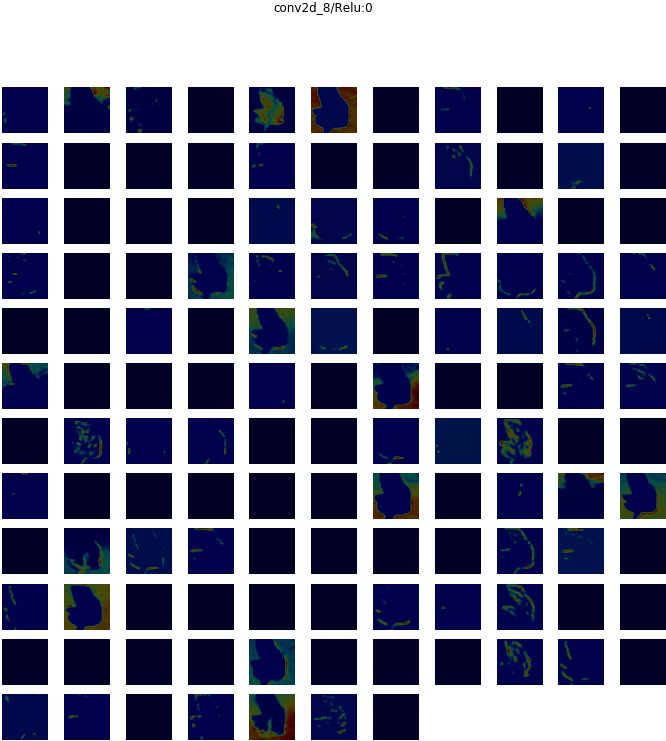
\includegraphics[width=\textwidth]{visualisierungen/yellow/heapmap_mit/conv2d_8.png}
	\caption{Visualisierung der Aktivierungswerte als Heatmap in der dritten Faltungschicht von dem TYLCV-Virus (eigene Darstellung).}
	\label{yellow_heat_vis}
\end{figure}



\newpage
\subsection{Samtfleckenkrankheit}

\begin{wrapfigure}{r}{7cm}
	\centering
	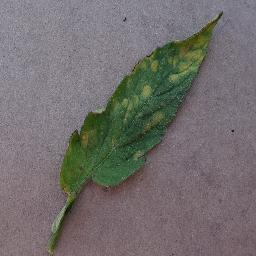
\includegraphics[width=0.45\textwidth]{visualisierungen/leaf_mold/mold_sample.jpg}%
	\caption{Das Beispielbild für die Visualisierung der Samtfleckenkrankheit (eigene Darstellung).}
	\label{mold_sample}
\end{wrapfigure}


In der Abbildung \ref{mold_sample} ist ein Blatt mit der Samtfleckenkrankheit abgebildet. Sehr viele gelbe Flecken sind in der Spitze des Blattes konzentriert. Im Inneren des Blattes auf der mittleren Höhe sind einige Ausprägungen sichtbar. Das Modell reagiert jeweils auf den linken und rechten Rand des Blattes. Die Abbildung \ref{mold6_act_vis} präsentiert deutlich, dass in der dritten Faltungschicht die Ausprägungen in der oberen Spitze nur von wenigen Filter angesprochen werden. In der vierten Faltungschicht (s. Abbildung \ref{mold8_anhang}) ist es zu abstrakt, um zu erkennen, ob das Modell das Verhalten der vorherigen Schicht übernommen hat. Des Weiteren zeigen in der dritten Faltungschicht 47 Filter keine Reaktion auf das Eingangsbild.

\begin{figure}[h!]
	\centering
	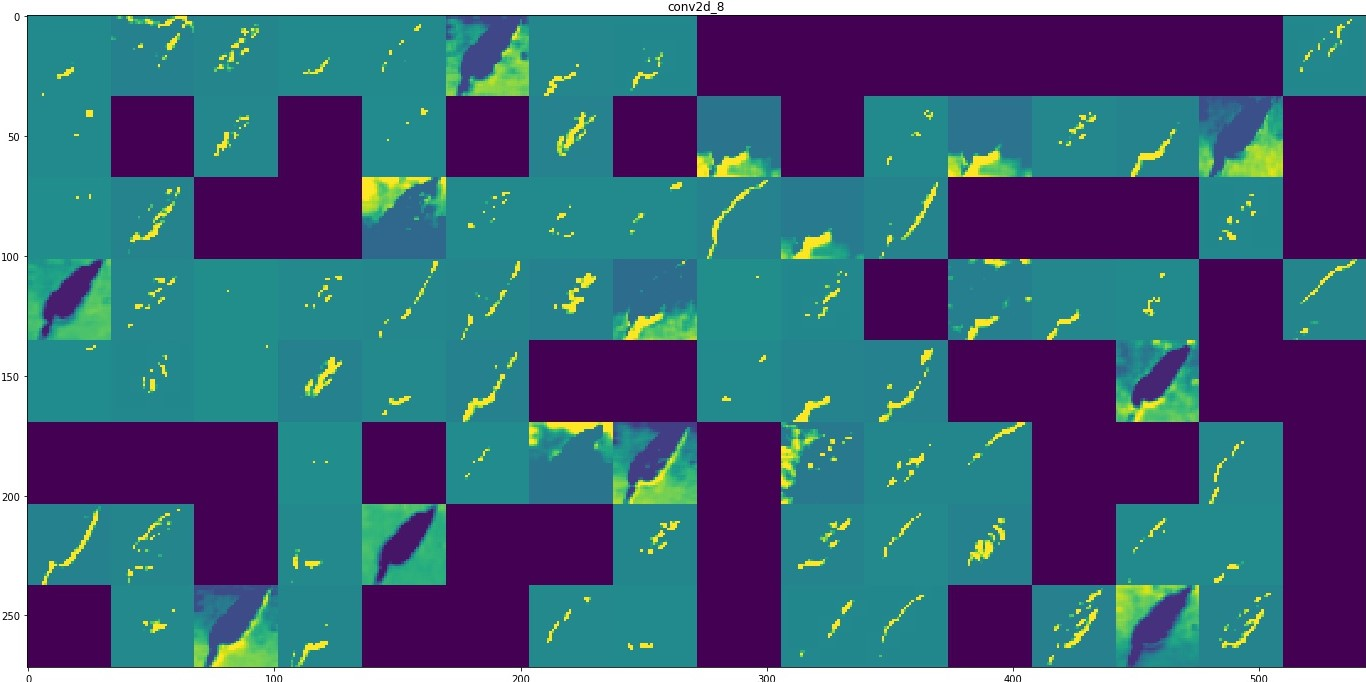
\includegraphics[width=\textwidth]{visualisierungen/leaf_mold/activation/mold6.JPG}
	\caption{Visualisierung der Aktivierungswerte in der dritten Faltungschicht von der Samtfleckenkrankheit (eigene Darstellung).}
	\label{mold6_act_vis}
\end{figure}
~\newline
Ein interessantes Merkmal, welches in den Aktivierungswerten nicht zu sehen ist, ist der horizontale Verlauf ausgehend von der Hauptaderung. Einige Filter in der Abbildung \ref{mold6_heat_vis} reagieren sehr stark darauf, zum Beispiel der Filter in der ersten Spalte und der sechsten Zeile. Des Weiteren sind die Ränder und die vorhin beschriebenen Positionen der Flecken relevant für das Modell. Dennoch lernt das Modell einige Male den Hintergrund.

\begin{figure}[h!]
	\centering
	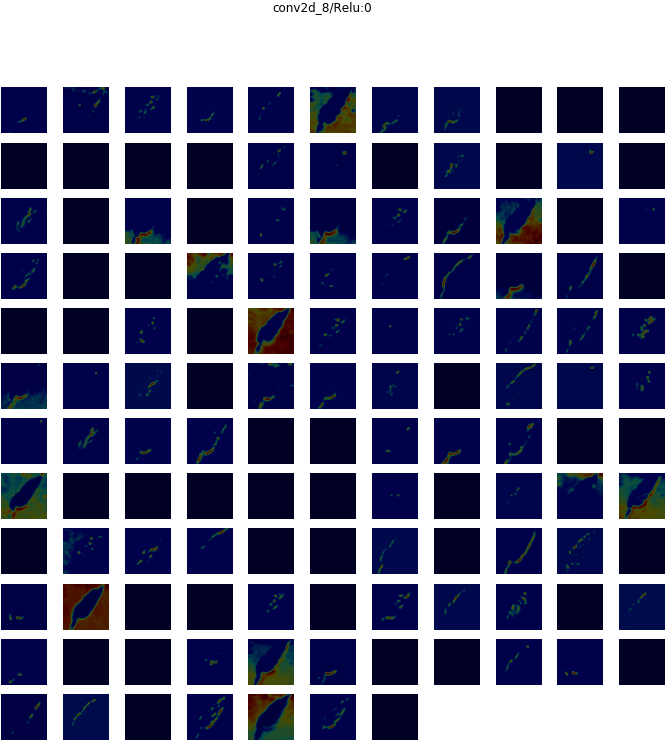
\includegraphics[width=\textwidth]{visualisierungen/leaf_mold/heatmap_mit/conv2d_8.png}
	\caption{Visualisierung der Aktivierungswerte als Heatmap in der dritten Faltungschicht von der Samtfleckenkrankheit (eigene Darstellung).}
	\label{mold6_heat_vis}
\end{figure}



\newpage
\subsection{Krautfäule}

\begin{wrapfigure}{r}{7cm}
	\centering
	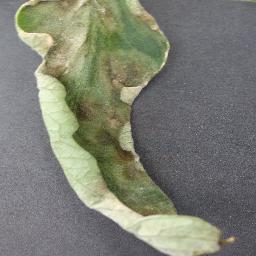
\includegraphics[width=0.45\textwidth]{visualisierungen/late/late_sample.jpg}%
	\caption{Das Beispielbild für die Visualisierung der Krautfäule (eigene Darstellung).}
	\label{late_sample}
\end{wrapfigure}


Das Beispielbild \ref{late_sample} veranschaulicht die typischen Ausprägungen von der Krautfäule. Diese zeichnen sich durch große braune Flecken aus. Um diese treten hellgrüne Verfärbungen auf, die das Blatt blass wirken lassen. Außerdem gibt es keine bevorzugte Position, auf der Ausprägungen auftreten. In der dritten Faltungschicht (s. Abbildung \ref{late6_act_vis}) ist zu erkennen, dass die Krümmung des linken Rands von dem Modell als interessantes Merkmal angesehen wird. Sehr viele Filter reagieren auf dieses Merkmal. Auch die Blattoberfläche ist für das Modell interessant. In der zehnten Spalte und der vierten Zeile sowie der sechsten Spalte und der ersten Zeile sind zwei Filter, die besonders auf die braune Ausprägung reagieren.


\begin{figure}[h!]
	\centering
	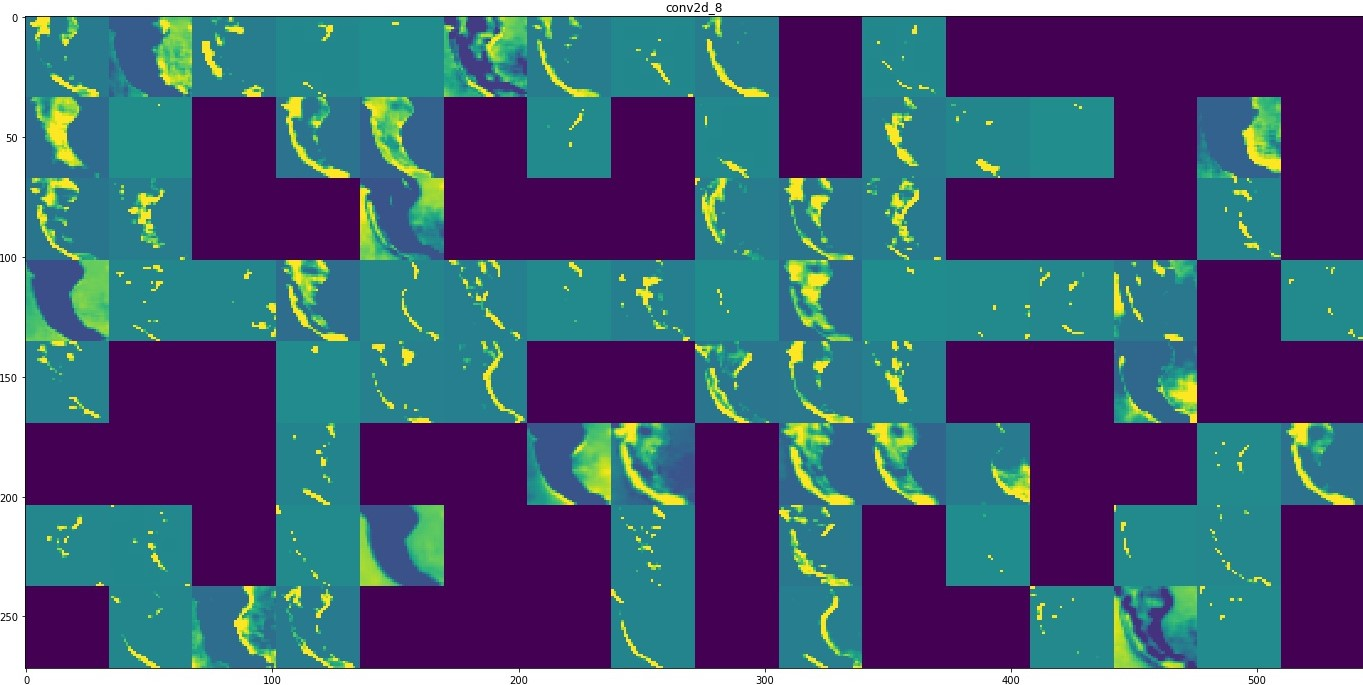
\includegraphics[width=\textwidth]{visualisierungen/late/activation/late_sample6.JPG}
	\caption{Visualisierung der Aktivierungswerte in der dritten Faltungschicht von der Krautfäule (eigene Darstellung).}
	\label{late6_act_vis}
\end{figure}
~\newline
Die Heatmap zeigt, dass die Beobachtungen mit den Aktivierungswerten übereinstimmen. Sehr viele konzentrierte Stellen treten auf diesem gekrümmten Rand auf. Darüber hinaus sind die Aktivierungswerte der drei großen braunen Flecken bei einigen Filtern konzentriert. Die Blattoberfläche mit der leichten blassen Verfärbung hat in der Abbildung \ref{late6_heat_vis} nur eine leichte Anhäufung von Aktivierungswerten. Insgesamt hat die dritte Faltungschicht 53 inaktive Filter.

\begin{figure}[h!]
	\centering
	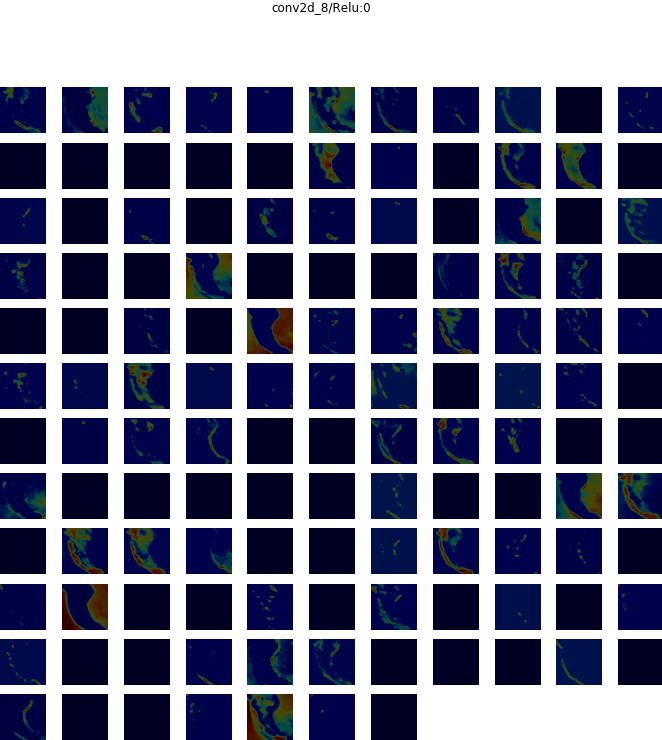
\includegraphics[width=\textwidth]{visualisierungen/late/heatmap_mit/conv2d_8.png}
	\caption{Visualisierung der Aktivierungswerte als Heatmap in der dritten Faltungschicht von der Krautfäule (eigene Darstellung).}
	\label{late6_heat_vis}
\end{figure}
